\documentclass[twocolumn]{article}
\usepackage[top=1.1in, left=0.85in, right=0.85in]{geometry}

\usepackage{amsthm}
\usepackage{relsize}
\usepackage{amsmath}
\usepackage{amssymb}
% \usepackage{code}
\usepackage{graphicx}
\usepackage{fancyvrb}
\usepackage{url}
\usepackage{textcomp}

\pagestyle{empty}

\newcommand\comment[1]{}

\newcommand\st{$^{\mathrm{st}}$}
\newcommand\nd{$^{\mathrm{nd}}$}
\newcommand\rd{$^{\mathrm{rd}}$}
\renewcommand\th{$^{\mathrm{th}}$}
\newcommand\tm{$^{\mbox{\tiny \textsc{tm}}}$}

% nice fractions
\newcommand\sfrac[2]{{}\,$^{#1}$\!/{}\!$_{#2}$}

\newcommand\citef[1]{\addtocounter{footnote}{1}\footnotetext{\cite{#1}}\ensuremath{^{\mbox{\footnotesize [\thefootnote]}}}}

\usepackage{ulem}
% go back to italics for emphasis, though
\normalem

\begin{document} 

\title{Snacking policies}
\author{Dr.~Tom~Murphy~VII~Ph.D.\thanks{
    Copyright \copyright\ 2016 the Regents of the Wikiplia Foundation.
    Appears in SIGBOVIK 2016 with the haunting memory of the
    Association for Computational Heresy; {\em IEEEEEE!} press,
    Verlag--Verlag volume no.~0x2016. ANG 0.00} }

\renewcommand\>{$>$}
\newcommand\<{$<$}

\date{1 April 2016}

\maketitle

\begin{abstract}
% XXX better abstract
what do I put here
\end{abstract}

\vspace{1em}
{\noindent \small {\bf Keywords}:
  snacking, consequentialism, comestability theory
}

\section{Introduction}

Some workplaces of the future now offer a feature called Snacks. With Snacks, a kitchenette is provided near workers, which supplies running water and an array of small food packs. These foods are free of (dollar) charge, but various spoken and unspoken rules govern worker interactions with the foods.

This presents a challenge, since some foods are more desirable than others. Specifically, say that one yogurt food comes in four varieties: Classic, Diet, Cherry-Vanilla, and Caffeine Free. Furthermore, say that one user \verb+<3+'s Cherry-Vanilla variety yogurt food and \verb+>=3+'s Caffeine Free variety yogurt food. This worker is happiest when he begins his office work while eating Cherry-Vanilla. If there is no Cherry-Vanilla, the worker may resort to Classic yogurt food, reducing his task-ready disposition, and thus performance. If all flavors have been exhausted but Caffeine Free, then the worker may take no yogurt at all, knowing that Caffeine Free brings more displeasure than even hunger. This creates a negative affect, which may cause the worker to actively sabotage the work of his peers. This provides poor Return on Investment (ROI).

One strategy is for this worker, who we will call Sal, to take all of the favored Cherry-Vanilla foods from the kitchenette to his desk at the beginning of the day. This strategy is called hoarding. This ensures that Sal may eat all his Cherry-Vanilla flavors. However, this behavior is considered unfair, for one reason that all other workers are completely deprived of Cherry-Vanilla flavor. It is perceived that Sal and all other workers should have equivalent access to the shared resource, except for the moment that he is selecting a food (for he is ``first in line,'' and lines are fair). Moreover, Sal should take only one food at a time (for it is ``Please help yourself. We ask that you take only one piece so that others may enjoy it as well,'' which is fair). We also perceive that Sal should take food only when he is actually hungry (for it is ``waste not, want not,'' and you can't spell ``aphorism'' without ``a fair is,'' mmm?).

Given these rules, there are still things that Sal can do to influence the chance that he gets the Cherry-Vanilla flavors. In particular, this paper investigates the strategy of Reordering, where Sal selects his favored snack, and also changes the order of the foods in the kitchenette. The thought is that while everyone retains equivalent access to the foods, other workers are less likely to select Cherry-Vanilla due to the decreased visibility and/or increased effort in finding them.

Note that the author does not reorder habitually reorder snacks; this question is of abstract philosophical interest. We consulted the wisdom of Judge John~Hodgman, who wrote~\cite{hodgman2016snacks}:

\begin{quotation}
  \noindent Why don't you just go out to lunch and buy the food you want with
  your own money?
  
  \noindent \ldots\ Stop with the personal e-mails and get back to work.
\end{quotation}

We did not find this to be a satisfactory argument.

\smallskip
In this paper, I first provide a short argument why Sal's behavior may be considered fair, using an unjustifiable but common assumption. I then give a formal model for Snacks, which can be used to conduct controlled experiments. I then show that under suitable conditions, Sal's behavior benefits both him and the workplace, in a Utilitarian sense.

\subsection{Game of Scones}

To investigate whether Reordering helps Sal and the rest of the workplace, we could run an experiment. Unfortunately this would be very expensive; we would need to find many workforces that are comparable, with similar food preferences, randomly assign some to the experimental group (where some fraction implement the Reordering policy) and then somehow judge their happiness. This would take a long time, and if the policy or experimental controls turn out to be harmful, might impact real GDP. For the effect sizes we see later, a live experiment is unlikely to show significance.

Instead, we develop a simple model that captures important aspects of the Snacks program, implement this on a computer, and then run millions of simulations.

The simplified model is as follows.

A simulation consists of an array $S$ of shelves, each of which is stocked with different varieties of food. The varieties are just given as integers from 0--$n_i$, where each food type (shelf) may have a different number of varieties. In an early version of the simulation each food and variety is given a name, so we might have a shelf consisting of many sodas, like\footnote{All of these brands now Copyright Trademark Patent Pending Dr.~Tom Murphy VII Ph.D., 2016!}

\begin{itemize}
\item Diet Kake 
\item Diet Thuck Lite
\item Mango Slooch 
\item Mr. Sleepe Black
\item Caffeine--Free Droob Ultra
\item Caffeine--Free Spask Black
\item Dr. Drarb Classic
\item Drorp Lite
\item Strawberry Sad 
\item Vanilla Grerb
\item Cherry Prote Lite
\item Diet Grobe
\item Dr. Brosh Lite
\item Duq Ultra
\item Grape Ding Lite
\item Mrs. Broop 
\item Diet Pap 
\item Grape Drax Classic
\end{itemize}

We also have an array $W$ of workers. Each worker has a preference function $P_{ij}$, one floating point value for each snack variety. This value may be negative, indicating an aversion to that snack. Nominally, these values are in dollars, for scale.

For simplicity, workers all get hungry at the same rate (although their hunger strikes randomly). When a worker hungers, she

\begin{enumerate}
\item Selects a shelf at random.
\item Sets her gaze upon the foremost variety on that shelf. She has some value $v$ for this item, given by $P$. \label{step:start}
\item She can see the number of items on the shelf, but not what varieties they are. From this number, she estimates what value $v'$ she would get from skipping the current variety (for this round) and setting her gaze upon the next one. \label{step:skip}
\item If $v' > v$, she does so, and repeats from step \ref{step:skip}.
\item If not, this is the food provisionally selected for this shelf, with value $v$.
\item If there are shelves remaining, she estimates the value of abandoning this shelf and trying the next one, $v''$.
\item If $v'' > v$, she moves to the next shelf and returns to step \ref{step:start}.
\item If she finishes with a selected food, she may reorder the items on the shelf of that food arbitrarily. She removes the selected food, if any, and eats it.
\end{enumerate}

No player retains any knowledge of the organization of a shelf between rounds.\footnote{This is not an accurate assumption in reality, but seems to only disadvantage those who reorder snacks from benefiting from their own treachery. A very advanced strategy might rearrange items on the shelf in order to encode information about what has been reordered, for example, by coding a specific unlikely pattern at the front of a shelf (or prior shelf) to foreshadow the hidden booty. Ultra-advanced strategies might place misleading codes to confuse other workers and cause them to make suboptimal choices. Hyper-advanced strategies might use steganographic techniques or cryptographic signatures to hide codes or make them tamper-proof. Of course, this does not matter in a real workplace because workers can remember extremely simple facts themselves.}

We have not yet said how the worker estimates the value of a shelf. But observe the following properties:

\begin{itemize}
\item If estimates are accurate, workers select a rational choice of food to maximize their own happiness.
\item If a user has a dramatically favored snack, she is willing to search deep within a shelf for it.
\item If a user has some snacks she favors and some she does not, she will be less willing to give up a good snack to find her favorite snack, because she might get stuck with a worse snack.
\end{itemize}

However, it also has an undesirable property:

\begin{itemize}
\item If a worker has a flat distribution of preferences, she will search the whole shelf. This is because there is no risk of getting stuck with a bad snack; she likes them all. This extends in a soft way to nearly flat distributions.
\end{itemize}

This does not match our intuitions of how real workers behave. Most of the time, an indifferent worker will just take a food that is ``good enough;'' this is known as ``satisficing.''\cite{simon1956rational} To prevent this, a worker's estimate of the value of continuing to search the shelf will include a small cost to search each item. This can be thought of as the cost of the physical labor or the displaced opportunity cost, or an estimate of the risk that an interruption causes her to have to stop searching before she selects a snack.

\medskip
The above requires an estimate of a shelf's value, both for the case where the worker may continue searching a shelf and the case where she continues to the next shelf. This can be computed with a recurrence relation. Since the worker cannot see beyond the snack her gaze is upon, this only depends on which shelf this is and the number of items on it. The expected value $E_s(n)$ for looking through $n$ items on shelf number $s$ is
%
$$
\begin{array}{c}
E_s(0) = 0 \\
E_s(n) = \mathlarger{\mathlarger{\sum}}_{i=1}^{V_s}\ \mathrm{P}(\mathrm{item}\ i) \times \mathrm{max}(P_{si}, E_s(n - 1) - c)
\end{array}
$$
%
where $V_s$ is the number varieties for shelf $s$, $\mathrm{P}(\mathrm{item}\ i)$ is the probability of selecting variety $i$ in the next slot, $P_{si}$ is the worker's preference for variety $i$ from shelf $s$, and $c$ is the small cost of looking at all. The content of the recurrence is simple: At each step, for each possible item, the worker can either can take that item with the value given by the preference function $P$, or keep going (but now there will be one fewer item).

Since we stipulate that the worker remembers nothing between rounds, the only probability distribution that makes sense for $\mathrm{P}(\mathrm{item}\ i)$ is the uniform one, so the general case becomes

$$
E_s(n) = \mathlarger{\mathlarger{\sum}}_{i=1}^{V_s}\ \frac{\mathrm{max}(P_{si}, E_s(n - 1) - c)}{V_s}
$$

Since this only depends on the preference function, we can compute this when the worker is born and print it on their birth certificate and employee badge.

\subsection{Experimenting}

I implemented the rules above in about 1000 lines of JavaScript,
including a UI, random number generation, and the experimentation harness.\footnote{It can be found at \url{sourceforge.net/p/tom7misc/svn/HEAD/tree/trunk/snacks/}.} 

Some other parameters need to be set: \verb+NUM_SHELVES+, \verb+NUM_PEOPLE+ and \verb+MAX_VARIETIES+, all self-explanatory; \verb+MIN_ITEMS+ and \verb+MAX_ITEMS+, the bounds on the number of snacks initially stocked per shelf (it seems that \verb+MIN+ should be at least 2, for the program is Snacks, plural); \verb+COST_TO_LOOK+, the penalty from the recurrence for estimating a shelf's value. We also have \verb+PREF_MEAN+ and \verb+PREF_STDDEV+ which are the parameters for the generation of preference functions (each is Gaussian---preferences are allowed to be negative). Finally, \verb+MEAN_WAIT+ gives the average amount of time between hunger events, wait times cannot be negative and so are distributed as $\Gamma(2.0, \verb+MEAN_WAIT+)$. We run each simulation for three eight-hour work days.

I then generated random scenarios and evaluated different snack
reordering policies. One extreme policy sorts the shelf in reverse
preference order, so that the worker's favorite snacks are at the
back. This seems unnecessary (takes $\mathrm{O}(n \mathrm{lg} n)$
time, unless perhaps using ``radix sort'') and unrealistic. It also
leads to substantial interference between workers, as one worker's
resorting completely undoes another's. Another relaxation of this,
more realistic, is where the worker only moves his favorite variety to
the depths of the shelf. This is analogous to a ``Move-to-Back
List''~\cite{rivest1976self}, except not really, since the worker
somehow finds all of the instances of their favorite variety in the
whole shelf before moving them to the back. The most realistic policy
generalizes this last one, and only moves the favorite snack when it
passes some ``outlier'' threshold for how much it is preferred over
the other snacks. This is the policy I ran many experiments for.

\medskip
The first thing to notice from the experiments is that the policy
doesn't even work! OMFG! For the reasonable parameter settings I
started with, not only is the overall happiness (value of snacks
eaten) neutral to slightly negative when the policy is in effect,
but the worker employing the reordering strategy \emph{also eats
  neutral to worse snacks}! This doesn't concur with anyone's
perspective on the problem (except maybe John~Hodgman's)---at least
the ``selfish'' worker who reorders snacks should be benefiting
from it, right?

Normally, this is where a heroic scientist would (a) implicate the
model, seeing as how it fails to have intuitive properties\footnote{I
  think that the model does not capture two important aspects. First
  is that Sal \emph{does know} that he's reordered the snacks and can
  likely find his favorites by just looking immediately to the back.
  Second is that traces of the model suggest that most workers look
  through nearly all of the snacks due to the (rational) expectation
  that they will improve their selection. There does not seem to be a
  good setting of the {\tt COST\_TO\_LOOK} penalty that suitably
  discourages workers from looking through the whole shelf while still
  allowing a resorter to find his deeply-placed favorites.} or (b)
give up. But owing to Draconian SIGBOVIK deadlines, this heroic
scientist resorts to another unjustifiable but common technique:
``Tweaking'' the model parameters until the experiments turn out as
expected (i.e., positive). Better yet, this process can be automated!

\medskip
Overnight in 4 separate browser tabs I ran a simple ``hyper-parameter
search'' to try to find the best settings of the parameters described
previously. I selected parameter values uniformly at random, and then
interpolated against the current local maximum (by averaging the
random point with the best point for each successive ``heads''
coin-flip during intialization). The goal was to find parameters that
simultaneously improved two scores in the experiment: The value of the
snacks eaten by the resorting worker, and the total value of snacks
eaten across all workers. (Specifically, I maximized the minimum of
these two). The best settings of the model had these values:

\begin{tabular}{@{\hspace{0.5in}}lr}
\verb+COST_TO_LOOK+ & 0.001 \\
\verb+MAX_ITEMS+ & 37 \\
\verb+MAX_VARIETY+ & 4 \\
\verb+MEAN_WAIT+ & 36305.715 \\
\verb+MIN_ITEMS+ & 3 \\
\verb+MRATIO+ & 1.010 \\
\verb+NUM_PEOPLE+ & 2 \\
\verb+NUM_SHELVES+ & 15 \\
\verb+OUTLIER_RATIO+ & 2.199 \\
\verb+PREF_MEAN+ & 1.320 \\
\verb+PREF_STDDEV+ & 5.625 \\
\end{tabular}

This an interesting instance: There are only two workers, but lots of
shelves and lots of snacks. Most interestingly, the mean hunger time is very unusually large (in the highest 97th percentile of the probability distribution): 36,305~seconds is over 10~hours! This means that in the course of a three-day simulation, we only expect each player to eat about 2.5~times. There is a very good chance that the workers never interact (never visit the same shelf) and more than a \sfrac{1}{4} chance that a worker never eats anything.

Repeating many more simulations with these parameter values
suggests---but does not prove---that this may just be a nearly
degenerate case in the simulation where the policies of the workers do
not matter, and what we are seeing is pure noise. However, when I
stopped the simulation arbitrarily after 1 million rounds, it produced
nice smooth-looking distributions, consistent with a good sample size
(Figure~\ref{figure:smooth}). The player implementing the resorting
policy ate 0.015\% better snacks on average, and the overall workplace
ate 0.031\% better snacks on average! This truly is a victory for
snack reordering and the scientific method! \qed

\begin{figure*}[p]
\begin{center}
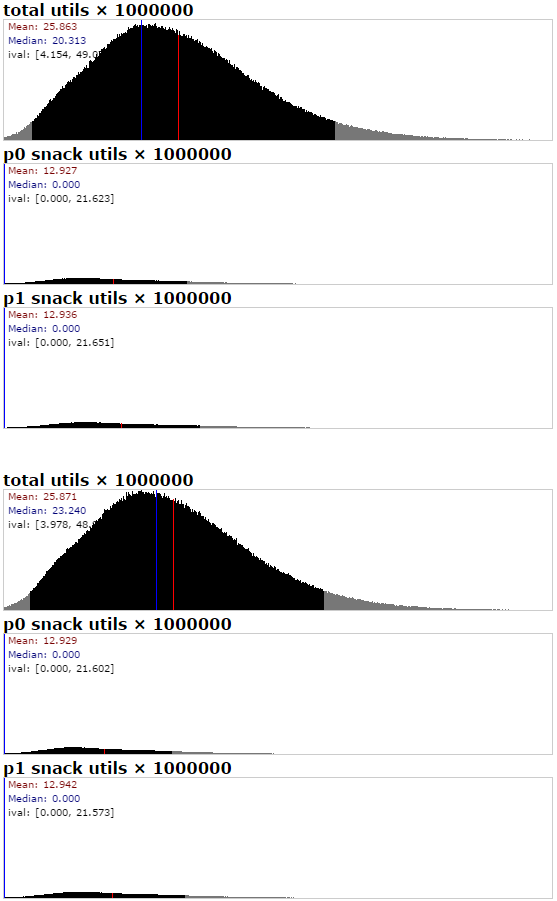
\includegraphics[width=3.5in]{utils}
\end{center}\vspace{-0.1in}
\caption{Histogram of one million experiments.} \label{figure:smooth}
\smallskip
The top group is the
  control (no resorting) and the bottom is the experiment (worker 0
  moves his favorite to the back of the shelf if its value exceeds the
  outlier ratio). Note how smooth the simulated outcomes are. This
  kind of graph is just the kind of statistics you write home about.
  Within each group, the big lump is the total snacks eaten by the two
  workers, and then the snacks eaten by each worker individually. Note
  a dramatic peak at the value 0 for the two workers, corresponding to
  {\it no snacks}; this happens because of the extreme hunger inteval
  of 10~hours. A overall value of zero is very unlikely because the
  simulation can only advance time (and thus end) when a worker has a
  chance to eat. Each histogram shows its mean and median, as well as
  darkening the 95\% highest density
  interval~\cite{kruschke2014doing}. An advanced technique would
  difference the values of the experiment and control and show a
  distribution of that statistic, but again, Draconian SIGBOVIK page
  size limitations preclude this. Normally we would use the 95\%
  intervals to make the comparison between control and experiment, but
  this appears to be unreadable due to the very smooth, nice looking
  distribution occluding it. Therefore we compare the means, seeing
  0.031\%, 0.015\%, and 0.046\% improvement in snack consumption
  respectively for the three pairs. Note that resorting is actually
  {\it altruistic} in this experiment, helping most the worker who does not
  sort! 

  \smallskip
  
  Without getting into too much math, regarding the frequentist
  standard of statistical significance typically used, we can say with
  confidence that $p > 0.05$.
% } 
\end{figure*}

  \comment{
--------------------------------------------------------------------------------



308000 rounds
Without reordering, utils: [589.02, 780.55] mean 684.87

Player 0 always sorts from the shelf he takes:

% 315000 rounds
% utils: [589.57, 792.09] mean 684.96
% p0: [9.11, 36.71] mean 22.59
% ineq: [20.34, 41.60] mean 30.60

total: 684.73 mean, 585.76--781.39
p0: 22.58, 8.82--36.77
ineq: 30.59, 19.93--41.84

No resorting:
total: 685.02 mean, 586.49--781.99
p0: 22.86, 9.50--37.97
ineq: 30.60, 19.92--41.79

Everyone resorts:
total: 684.46 mean, 586.26 -- 780.25
p0: 22.83 mean, 8.96-37.40
ieq: 30.55 19.94--41.27


--------------------

with 0.05 cost to look

total utils: 594.49 mean, 509.82-681.81
p0: 19.83 mean, 7.22-33.24
ieq: 28.07, 18.30-38.49

only p0 sorts:
total utils: 585.52 mean, 499-669
p0: 18.65 7.07-31.26
ieq: 27.92 18.33-38.38



Everyone puts favorite last:
total: 546.61 [466.36, 626.97]
p0: 18.24 [6.39, 31.27]
ieq: 26.92 [17.73, 37.05]


--------------------------------------------------
Now using 100k iterations. everyone puts snack last:

snacks at end × 100000 = Mean: 201.47 [116.62 , 443.72] Median: 208.81
total utils × 100000 = Mean: 546.75 [466.20 , 625.91] Median: 539.81
p0 utils × 100000 = Mean: 18.24 [6.06 , 30.91] Median: 16.52
inequality × 100000 = Mean: 26.91 [17.90 , 37.38] Median: 25.14

nobody sorts:
snacks at end × 100000 = Mean: 201.65 [116.65 , 421.74] Median: 217.99
total utils × 100000 = Mean: 594.17 [508.66 , 680.64] Median: 590.98
p0 utils × 100000 = Mean: 19.82 [7.52 , 33.50] Median: 19.63
inequality × 100000 = Mean: 28.05 [18.23 , 38.42] Median: 26.23

we eat almost exactly the same number of snacks, but are less happy.


nobody sorts; measure snack utils specifically:

snacks at end × 100000 = Mean: 201.26 [116.59 , 417.74] Median: 203.90
total utils × 100000 = Mean: 594.45 [506.68 , 679.40] Median: 588.88
p0 utils × 100000 = Mean: 19.83 [7.53 , 33.60] Median: 17.61
p0 snack utils × 100000 = Mean: 22.30 [8.49 , 36.57] Median: 20.62
inequality × 100000 = Mean: 28.05 [18.31 , 38.37] Median: 26.00

only p0 sorts:

snacks at end × 100000 = Mean: 201.52 [117.71 , 421.74] Median: 198.99
total utils × 100000 = Mean: 590.13 [507.03 , 678.05] Median: 590.58
p0 utils × 100000 = Mean: 18.98 [7.34 , 31.92] Median: 18.44
p0 snack utils × 100000 = Mean: 22.19 [9.17 , 37.02] Median: 20.87
inequality × 100000 = Mean: 27.99 [18.52 , 38.53] Median: 25.96

only p0 places outliers:

snacks at end × 100000 = Mean: 201.54 [117.79, 435.73] Median: 198.50
total utils × 100000 = Mean: 592.27 [509.32, 681.56] Median: 593.03
p0 utils × 100000 = Mean: 19.48 [7.14, 32.58] Median: 17.97
p0 snack utils × 100000 = Mean: 22.28 [8.53, 36.59] Median: 19.70
inequality × 100000 = Mean: 28.01 [18.51, 38.60] Median: 27.01



Credible interval\cite{kruschke2014doing}
}

\bibliographystyle{IEEEtran}
% \bibliographycomment{} % nothing
\bibliography{paper}

\end{document}
